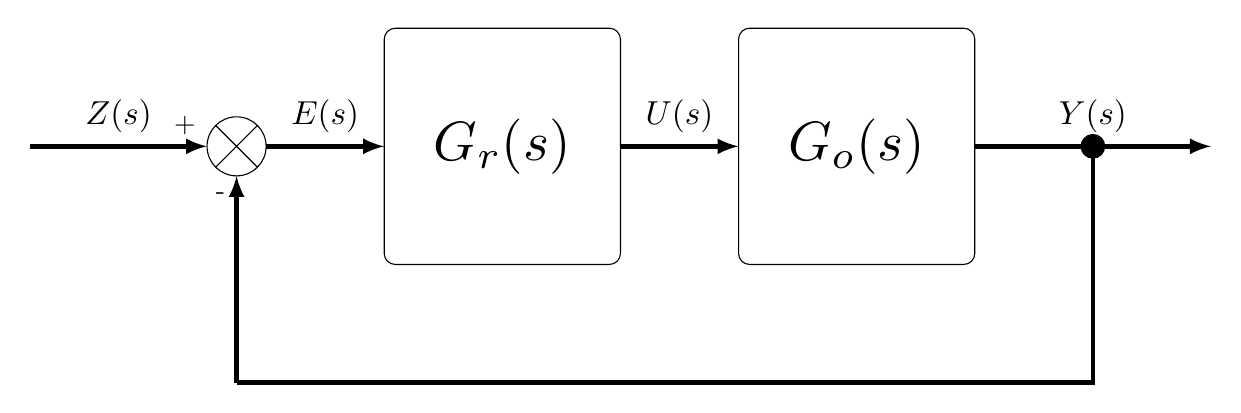
\begin{tikzpicture}[scale=1.5]
	\draw[-latex, ultra thick]
		(0,0)	--	node[scale=1.2,above]{$Z(s)$}
		(1.5,0)	node[above left]{+};
	\draw
		(1.75,0)	circle (0.25)
		+(45:0.25)	--
		+(-135:0.25)
		+(-45:0.25)	--
		+(135:0.25);
	\draw[-latex, ultra thick]
		(1.75,-2)	--
		(1.75,-0.25)	node[below left]{-};
	\draw[-latex, ultra thick]
		(2,0)	--	node[scale=1.2,above]{$E(s)$}
		+(1,0);
	\draw[rounded corners]
		(3,-1)	rectangle
		+(2,2)
		+(1,1)	node[scale=2]{$G_r(s)$};
	\draw[-latex, ultra thick]
		(5,0)	--	node[scale=1.2,above]{$U(s)$}
		+(1,0);
	\draw[rounded corners]
		(6,-1)	rectangle
		+(2,2)
		+(1,1)	node[scale=2]{$G_o(s)$};
	\draw[-latex, ultra thick]
		(8,0)	--	node[scale=1.2,above]{$Y(s)$}
		+(2,0);
	\draw[ultra thick]
		(9,0)		--
		++(0,-2)	--
		++(-7.25,0);
	\filldraw[color=black]
		(9,0) circle (0.1);
	
\end{tikzpicture}